\documentclass[../main/main.tex]{subfiles}

\newdate{date}{04}{12}{2019}


\begin{document}

\marginpar{ \textbf{Lecture 15.} \\  \displaydate{date}. \\ Compiled:  \today.}



This first approximation is reasonable if either
\begin{enumerate}
\item \( \rho  \) is small enough. It implies that \( \abs{\va{r}_i - \va{r}_j} \gg 1 \) and hence \( \Phi _{ij} \ll 1 \).
\item Sufficiently high \( T \) such that \( \Phi (\abs{\va{r}_i - \va{r}_j} )/k_B T \ll 1 \). What is important it is the ration between \( \beta  \)  and \( \Phi _{ij} \).
\end{enumerate}
In either cases we have \( \exp (- \beta \Phi _{ij}) \rightarrow 1 \) and \( f_{ij} \rightarrow 0 \). By keeping only linear terms the partition function is
\begin{equation}
\begin{split}
  Q_N (V,T) &= \int_{V}^{} \dd[]{\va{r}_1} \dots \dd[]{\va{r}_N} \qty(1+ \sum_{i,j>i}^{} f_{ij} + \dots )  \\
  &= V^N + \sum_{i,j>i}^{} \int_{V}^{} \dd[]{\va{r}_1} \dots \int_{V}^{}  \dd[]{\va{r}_N} f_{ij} \\
  &= V^N + V^{N-2} \sum_{i,j>i}^{} \int_{V}^{} \dd[]{\va{r}_i} \dd[]{\va{r}_j} f_{ij} + \dots \\
\end{split}
\end{equation}
We are summing up over all configurations \( ij \). Let us try to compute the double integral:
\begin{equation}
  \int_{V}^{} \dd[]{\va{r}_i} \dd[]{\va{r}_j} f_{ij} (\abs{\va{r}_i - \va{r}_j} ) \underset{\substack{ \text{translational} \\  \text{symmetry} } }{=}  \int_{}^{} \dd[]{\va{r}_i} \dd[]{\va{r}_j} f (\va{r})
  = V \int_{V}^{} \dd[]{\va{r}}  f \qty(\abs{\va{r}} ) \equiv -2 B_2 V
\end{equation}
where
\begin{equation}
  B_2 \equiv - \frac{1}{2} \int_{V}^{} \dd[]{\va{r}}  f \qty(\abs{\va{r}} )
\end{equation}
so, what is important it is the relative distance. \( \va{r} \) gives us the position from the center we have choosen.
Rewriting again the partition function we obtain:
\begin{equation}
  Q_N (V,T) = V^N - V^{N-1} N (N-1) B_2 (T)
\end{equation}
\begin{remark}
The factor \( \frac{N(N-1)}{2} \) comes out becouse in the double sum are considered all the possible connections (bonds) between pairs of particles \( (i,j) \) with \( j>i \).
\end{remark}
\begin{equation}
  Z_N (V,T) = \qty(\frac{V^N}{N! \Lambda ^{3N}}) \qty(1- \overset{N(N-1) \approx N^2}{\frac{N^2}{V}} B_2 (T)+ \dots)
\end{equation}
\begin{remark}
We do not care about the \( (N-1) \) term, because \( N \) is big enough!
\end{remark}
The free energy is:
\begin{equation}
  F_N = F_N^{ideal} - k_B T \ln{\qty[1-\frac{N^2}{V}B_2 (T)+ \dots] }
\end{equation}
Hence,
\begin{equation}
  P_N = - \qty(\pdv{F_N}{V} )_{T,N} = \frac{N k_B T}{V} \qty(1+ \frac{\frac{N}{V}B_2}{1- \frac{N^2}{V}B_2})
  = \frac{N k_B T}{V} \qty(\frac{1 -\frac{N^2}{V} B_2 + \frac{N}{V} B_2 }{1- \frac{N^2}{V} B_2})
\end{equation}
Expanding the denominator for \( \frac{N}{V} B_2 \ll 1 \) \( \rho \ll 1 \) one gets
\begin{equation}
  P_N \simeq \frac{N k_B T}{V} \qty(1+\frac{N}{V}B_2 + \dots)
  \label{eq:15_1}
\end{equation}
here we see the ideal gas and the correction to the ideal gas.
\begin{remark}
The equation \eqref{eq:15_1} gives an important relation between experimentally accessible observables as \( P_N \) and microscopic quantities such as \( f(\va{r}) \) (and hence \( \Phi (\va{r}) \)) trough the estimate of \( B_2 \).

Therefore, it is important computing \( B_2 \), because one time we have this we have the expansion. Or if we wish, by doing the fit of data at different temperature we obtain \( B_2 \) from the experiment and we can see \( f_{ij} \).
\end{remark}
\begin{remark}
The virial expansion obtained in \eqref{eq:15_1} is valid for small densities.
\end{remark}


To consider higher order terms in the virial expansion we need to consider higher order products of the \( f_{ij} \).

Before doing this, however, one can show that an higher order expansion can be obtained by using the following (rather rude) trick.

Since \(  (1-x)^{-1} = 1 + x + \dots \), ny going backward it is possible to write
\begin{equation}
  \frac{PV}{N k_B T} \approx 1 + \rho B_2 + \dots \simeq \frac{1}{1-B_2 \rho }
\end{equation}
this is the Clausius equation. On the other hand,
\begin{equation}
  \frac{1}{1-B_2 \rho } \simeq  1 + B_2 \rho + \underbrace{(B_2)^2 \rho ^2}_{B_3 \approx B_2^2}  + \underbrace{(B_2)^3 \rho ^3}_{B_4 \approx B_2^3} + \dots
\end{equation}
Identifying the coefficients for each power we get, for example
\begin{equation}
  B_3 \approx (B_2)^2, \quad B_4 \approx (B_2)^3
\end{equation}
This is the approximation of higher order virial coefficients with powers of \( B_2 \).
\begin{example}
Exam: let us compute virial expansion of a gas in a potential.
\end{example}

\subsection{Computation of \( B_2 \) for given \( \Phi  \)}
\subsubsection{Gas of hard spheres}
The particles are interacting (it is not ideal!) and there is a size that is the range of the potential.
\begin{equation}
  \Phi (r) = \begin{cases}
    \infty & r < \sigma \\
    0     & r \ge \sigma
\end{cases}
\end{equation}
\begin{figure}[h!]
\centering
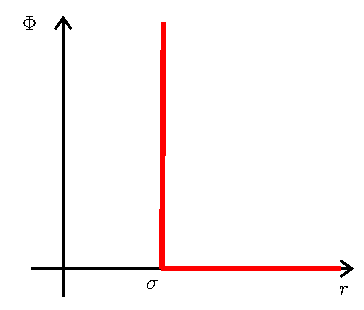
\includegraphics[width=0.5\textwidth]{../lessons/15_image/1.pdf}
\caption{\label{fig:} Plot of the potential \( \Phi (r) \).}
\end{figure}
Hence,
\begin{equation}
  e^{-\beta \Phi (r)} = \begin{cases}
    0 & r < \sigma\\
    1 & r \ge \sigma
  \end{cases}
\end{equation}
This implies that
\begin{equation}
  B_2 (T)= - \frac{1}{2} \int_{V}^{} \dd[]{\va{r}}  f \qty(\abs{\va{r}} )
  = - \frac{1}{2} 4 \pi \int_{V}^{} \dd[]{r} r^2 \qty[e^{-\beta \Phi (r)}-1 ]
  = 2 \pi \int_{0}^{\sigma } \dd[]{r} r^2 = \frac{2}{3} \pi  \sigma ^3
\end{equation}
\begin{equation}
  \Rightarrow B_2^{HS} (T) = \frac{2}{3} \pi  \sigma ^3
\end{equation}
this is the second virial coefficient for a hard sphere gas. There is no condensation in the gas spheres.
\begin{remark}
As expected \(  B_2^{HS} \) does not depend on temperature (purely repulsive interaction).
\end{remark}
For hard spheres we have:
\begin{equation}
  P V = N k_B T \qty(1 + \frac{2}{3} \pi \sigma ^3 \frac{N}{V})
\end{equation}
\begin{remark}
The excluded volume interaction (hard sphere) increases the product \( PV \) with respect to the ideal gas.
\end{remark}

Let us say, that the potential is not anymore zero but is \( - \varepsilon  \) when it is in the case \( r \ge \sigma \). Or consider a case in which it is \( - \varepsilon  \) between \( [\sigma ,2 \sigma ] \), then it goes to zero.
\subsubsection{Gas with Lennard-Jones interaction}
We can consider a Lennard-Jones potential. The 2-body Lennard-Jones potential energy is
\begin{equation}
  \Phi = 4 \varepsilon \qty[\qty(\frac{\sigma }{r})^{12} - \qty(\frac{\sigma }{r})^6  ]
\end{equation}
where the first one is the repulsive term (Pauli excluded principle) and the second is the attractive term (fluctuation of the elecrtic dipole moment).

\begin{figure}[h!]
\centering
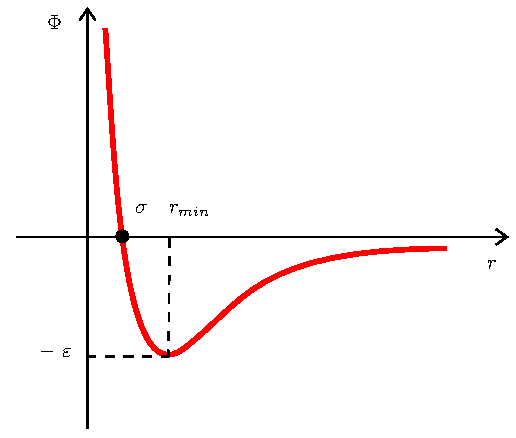
\includegraphics[width=0.5\textwidth]{../lessons/15_image/2.pdf}
\caption{\label{fig:} Plot of the Lennard-Jones potential.}
\end{figure}
 The minimum is in \( r_{min}=2^{1/\sigma } \).   You can play with the range of attraction by changing \( \sigma  \) or by changing the   \( \varepsilon  \).
 What it is important is that for the Lennard-Jones we have
 \begin{equation}
   B_2 \overset{LJ}{=} B_2 (T)
 \end{equation}
\begin{equation}
  B_2 (T) = - 2 \pi \int_{0}^{\infty } r^2 \qty[e^{- \frac{4 \varepsilon }{k_B T} \qty[\qty(\frac{\sigma }{r})^{12} - \qty(\frac{\sigma }{r})^6] } -1] \dd[]{r}
\end{equation}
It is not solvable exactly but by series expansion. Let us consider the following change of variables
\begin{equation}
  x = \frac{r}{\sigma }, \quad \tau = \frac{k_B T}{\varepsilon }
\end{equation}
Integrating by parts \( \int_{}^{} f' g = fg - \int_{}^{} g' f    \) where \( f' = x^2 g = \exp [-()]   \), we obtain
\begin{equation}
\begin{split}
  B_2 (T^*) &= \frac{2}{3} \pi \sigma ^3 \frac{4}{\tau } \int_{0}^{\infty } x^2  \qty(\frac{12}{x^{12}}- \frac{6}{x^6}) e^{- \frac{4}{\tau } \qty(\frac{1}{x^{12}} - \frac{1}{x^6}) }  \dd[]{x}  \\
  & = A \int_{0}^{\infty } \qty(\frac{12}{x^{16}}- \frac{6}{x^4}) e^{- \frac{4}{\tau } \qty(\frac{1}{x^{12}} - \frac{1}{x^6}) } \dd[]{x}
\end{split}
\end{equation}
Expand the exponential and then integrate term by term. One gets a serie in inverse power of \( \tau  \).
\begin{equation}
  B_2 (\tau ) = - 2 A' \sum_{n=0}^{\infty } \frac{1}{4n!} \Gamma \qty(\frac{2n-1}{4}) \qty(\frac{1}{\tau })^{\frac{2n+1}{4}}
\end{equation}
where \( \Gamma  \) is the Euler function.
\begin{remark}
Note that, because the Lennard-Jones potential has an attractive interaction term \( \qty[- \qty(\frac{\sigma }{r})^6 ]  \), the second virial coefficient depends on temperature.
\end{remark}
\subsection{Higher order terms in the cluster expansion}
Let us consider again the formal expansion
\begin{equation}
  \prod_{i}^{} \qty(\prod_{j>i}^{} (1+f_{ij}) ) = 1 + \sum_{i,j>i}^{} f_{ij}
  + \sum_{\substack{ i \\ j>i \\ l>k \\ k \ge i \\ (ij) \neq (kl)} }^{} f_{ij} f_{kl}     + \dots
\end{equation}
The problem with this expansion is that it groups terms quite different from one another. Fro example the terms \( f_{12}f_{23} \) and \( f_{12}f_{34} \). Indeed the first term correspond to a diagram as in Figure \ref{fig:15_1_1}, while the second to two disconnected diagrams as in Figure \ref{fig:15_1_2}.
\begin{figure}[h!]
\begin{minipage}[c]{0.5\linewidth}
\subfloat[][Description]{ 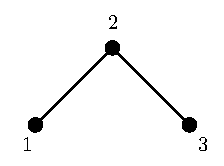
\includegraphics[width=0.6\textwidth]{../lessons/15_image/3.pdf}  \label{fig:15_1_1} }
\end{minipage}
\begin{minipage}[]{0.5\linewidth}
\centering
\subfloat[][Description]{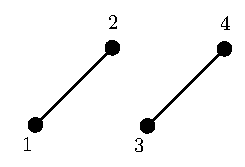
\includegraphics[width=0.6\textwidth]{../lessons/15_image/4.pdf}  \label{fig:15_1_2} }
\end{minipage}
\caption{\label{fig:} }
\end{figure}

Another problem of the above expansion is that it does not recognize identical clusters formed by different particles. For example the terms \( f_{12} f_{23} \) and \( f_{12}f_{14} \) contribute in the same way to the partition function. It is then convenient to follow a diagrammatic approach similar to the Feymann approach in the reciprocal space.

\begin{minipage}[c]{0.7\linewidth}
For the linear term \( f_{ij} \) the only diagram is given by Figure \ref{fig:15_2}. As we have seen this has multeplicity \( \frac{N(N-1)}{2} \) and the integral is of the form
\begin{equation}
  \int_{}^{}  f_{12} \dd[]{\va{r}_1} \dd[]{\va{r}_2}  = V \int_{}^{} f(\va{r}) \dd[]{\va{r}}  = - 2 V B_2
\end{equation}
\end{minipage}
\begin{minipage}[]{0.3\linewidth}
\centering
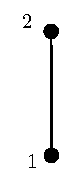
\includegraphics[width=0.3\textwidth]{../lessons/15_image/5.pdf}
\captionof{figure}{\label{fig:15_2} }
\end{minipage}

\begin{minipage}[c]{0.7\linewidth}
For the term \( f_{ij}f_{kl} \) we can have the case as in Figure \ref{fig:15_3},
that has molteplicity
\begin{equation}
  \frac{N(N-1)}{2} \frac{(N-1)(N-3)}{2} \frac{1}{2}
\end{equation}
 and the integral is of the  form
\begin{equation}
  \int_{}^{}  f_{12} f_{34} \dd[]{\va{r}_1} \dd[]{\va{r}_2}  \dd[]{\va{r}_3}  \dd[]{\va{r}_4}
\end{equation}
i.e. involving 4-particles
\begin{equation}
\begin{split}
 &  \int_{}^{}  f( \abs{\va{r}_1 - \va{r}_2} )f( \abs{\va{r}_3 - \va{r}_4} ) \dd[]{\va{r}_1}  \dd[]{\va{r}_2}  \dd[]{\va{r}_3}  \dd[]{\va{r}_4}
  = \\
  & = V^2 \qty(\int_{}^{} f(\va{r})\dd[]{\va{r}}  )^2 = 4 V^2 B_2^2
\end{split}
\end{equation}
\end{minipage}
\begin{minipage}[]{0.3\linewidth}
\centering
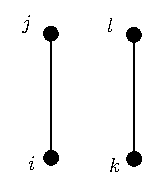
\includegraphics[width=0.6\textwidth]{../lessons/15_image/6.pdf}
\captionof{figure}{\label{fig:15_3} }
\end{minipage}

\begin{minipage}[c]{0.7\linewidth}
The next case if for instance as in Figure \ref{fig:15_4}. This involves 3 particles.
The multiplicity of this diagram is
\begin{equation}
  \frac{N (N-1) (N-2)}{3!} \times 3
\end{equation}
The integral is of the form
\begin{equation}
\begin{split}
  & \int_{}^{}  f_{12} f_{23} \dd[]{\va{r}_1}  \dd[]{\va{r}_2}   \dd[]{\va{r}_3}
  \simeq V  \qty(  \int_{}^{} \dd[]{r} f(r)  )^2  = \\
  & =   \int_{}^{}  f( \abs{\va{r}_1 - \va{r}_2} )f( \abs{\va{r}_2 - \va{r}_3} ) \dd[]{\va{r}_1}  \dd[]{\va{r}_2}  \dd[]{\va{r}_3}  = \\
  & = V \qty(\int_{}^{} f(\va{r})\dd[]{\va{r}}  )^2  = 4 V B_2^2
\end{split}
\end{equation}
\end{minipage}
\begin{minipage}[]{0.3\linewidth}
\centering
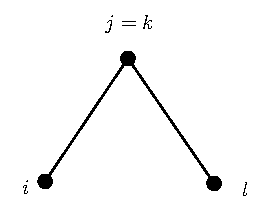
\includegraphics[width=0.8\textwidth]{../lessons/15_image/7.pdf}
\captionof{figure}{\label{fig:15_4} }
\end{minipage}

\begin{minipage}[c]{0.7\linewidth}
Another interesting diagram is the one in Figure \ref{fig:15_5}. Its molteplicity is
\begin{equation}
  \frac{N(N-1)(N-2)}{3!}
\end{equation}
The associated integral involves 3 particles and it is of the form
\begin{equation}
\begin{split}
   & \int_{}^{} f_{12} f_{23} f_{31} \dd[]{\va{r}_1}  \dd[]{\va{r}_2} \dd[]{\va{r}_3} = \\
   & = \int_{}^{} f ( \abs{\va{r}_1 - \va{r}_2} ) f ( \abs{\va{r}_2 - \va{r}_3} )  f ( \abs{\va{r}_3 - \va{r}_1} )  \dd[]{\va{r}_1} \dd[]{\va{r}_2} \dd[]{\va{r}_3} \\
   & = \int_{}^{} f ( \abs{\va{r}_1 - \va{r}_2} ) f ( \abs{\va{r}_2 - \va{r}_3} )  f ( \abs{\va{r}_3 - \va{r}_1} )  \dd[]{\va{r}_2} \dd[]{\va{r}_{21}} \dd[]{\va{r}_{23}}
\end{split}
\end{equation}
\end{minipage}
\begin{minipage}[]{0.3\linewidth}
\centering
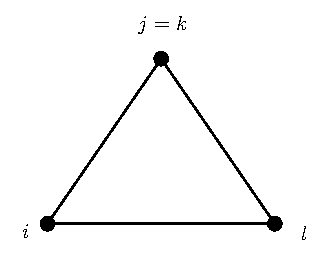
\includegraphics[width=0.8\textwidth]{../lessons/15_image/8.pdf}
\captionof{figure}{\label{fig:15_5} }
\end{minipage}
On the other hand \( \va{r}_{13} = \va{r}_{23} - \va{r}_{21} \), which implies
\begin{equation}
   f ( \abs{\va{r}_3 - \va{r}_1} )  =  f ( \abs{\va{r}_{23} - \va{r}_{21}} )
\end{equation}
hence,
\begin{equation}
  \int_{}^{} f (\abs{\va{r}_{12}} ) f (\abs{\va{r}_{23}} ) f (\abs{\va{r}_{31}} ) \dd[]{\va{r}_{21}}  \dd[]{\va{r}_{23}}  \dd[]{\va{r}_{2}}
  =
    \int_{}^{} f (\abs{\va{r}_{12}} ) f (\abs{\va{r}_{23}} ) f (\abs{\va{r}_{23}-\va{r}_{21}} )  \dd[]{\va{r}_{21}}  \dd[]{\va{r}_{23}}  \dd[]{\va{r}_{2}}
\end{equation}
Let us call this integral
\begin{equation}
  \int_{}^{} f_{12} f_{23} f_{31} \dd[]{\va{r}_1}  \dd[]{\va{r}_2}   \dd[]{\va{r}_3}
  \equiv  3! V  \qty( B_3 - 2 B_2^2  )
\end{equation}
The configurational partition function with these terms becomes
\begin{equation}
\begin{split}
Q_N (V,T) = &  V^N - V^N \frac{N(N-1)}{V} B_2 + V^N\frac{ N (N-1)(N-2)(N-3)}{8V^2} (4B_2^2)  \\
& + V^N \frac{N(N-1)(N-2)}{2V^2} 4B_2^2 \\
& = V^N \qty(1 + \frac{N(N-1)}{V} B_2 + \frac{N(N-1)(N-2)(N-3)}{2V^2} B_2^2 + \frac{N(N-1)(N-3)}{V^2} B_3)
\end{split}
\end{equation}
Let us now face the problem in a slightly different ways. Let us remind that
\begin{equation}
  Q_N (V,T) = \sum_{diagrams}^{} \int_{}^{} \prod_{kl}^{} f_{kl} \dd[3N]{r}
\end{equation}
i.e. sum over all possible diagrams i.e. all possible ways in which a can draw edges between pairs of points \( (k,l) \). 
\section{lesson}




\section{Landau mean field of phase transition}
Assumptions:
\begin{enumerate}
\item Existence of an order parameter \( \eta   \). Remember the definition of the order parameter:
\begin{equation}
  \eta   = \begin{cases}
    0 & T \ge \bar{T} \text{ (disordered or symmetric phase)}\\
    \neq 0 & T < \bar{T}  \text{ (ordered symmetry is broken)}
\end{cases}
\end{equation}
\item The \emph{free energy} is an analytic function of the order parameter \( \eta   \). It is because you are doing the expansion close to...etc etc. Therefore, \( \mathcal{L} = \mathcal{L} (\eta ) \).
\item Form of \( \mathcal{L} \) must satisfy the symmetries of the system.
\item Equilibrium states are the ones that minimise \( \mathcal{L} \). Absolute minima.
\end{enumerate}
\begin{equation}
  \mathcal{L} (\eta ) \approx a_0 + a_1 \eta + a_2 \eta ^2 + a_3 \eta ^3 + \dots
\end{equation}
In this case \( \eta  \) is scalar.

If \( \mathbb{Z}^2 \) symmetry we have:
\begin{equation}
  \mathcal{L} (-\eta ) =   \mathcal{L} (\eta )
\end{equation}

We are interested in the minima.
Since we want \( \eta = 0 \) to be a solution we want \( a_1 = 0,a_3= 0 \dots \).
Therefore, in \( \mathbb{Z}^2 \) symmetry:
\begin{equation}
  \mathcal{L} (\eta ) \simeq a_0 + a_2 \eta  ^2 + a_4  \eta  ^4 + O(\eta ^6)
\end{equation}
\begin{subequations}
\begin{align}
  a_0 &= a_0 (J,T) \\
  a_2 &= a_2 (J,T) \\
  a_4 &= a_4 (J,T)
\end{align}
\end{subequations}
if \( T > \bar{T}  \), \( \eta =0 \) it implies \( \mathcal{L} (\eta = 0) = a_0 \). Therefore,
\begin{equation}
    \mathcal{L} (\eta ) \simeq  a_2 \eta  ^2 + a_4  \eta  ^4
\end{equation}
The term \( a_4 \) it is positive and fixed.

Expand in \( t \equiv \frac{T - \bar{T} }{\bar{T} } \), when \( T = \bar{T} \rightarrow a_2 = 0 \).
The Landau free energy in the minimal form is:
\begin{equation}
  \mathcal{L} =  \mathcolorbox{green!20}{\frac{a}{2}} t \eta ^2 + \frac{b}{4} \eta ^4
\end{equation}
\begin{remark}
does not matter the coefficient in green in front, so in the next part of the course we will change it. If it is written in this way we have always \( a>0 \). We have also \( b>0 \).
\end{remark}
For the Gibbs version (that can be useful):
\begin{equation}
  \mathcal{L} =  \mathcolorbox{green!20}{\frac{a}{2}} t \eta ^2 + \frac{b}{4} \eta ^4 - h \eta
\end{equation}
we insert a field coupled with the order parameter.

Suppose to look for \( h=0 \), the equilibrium states are the minima
\begin{equation}
  \pdv{\mathcal{L}}{\eta } = 0 \quad \Rightarrow  a t \eta + b \eta ^3 = 0
\end{equation}
so
\begin{equation}
  \eta (at+b \eta ^2) ) 0 \quad \Rightarrow \eta =0, \eta = \pm \sqrt{\frac{-at}{b}}
\end{equation}
(insert plot of \( (\eta,\mathcal{L}) \) for \( t>0 \)  and \( t<0 \) ).

The solutions in the case \( t<0 \) are correlated by the \( \mathbb{Z}^2 \) symmetry.
The free energy is like the: (plot of \( x^4 \) ..... vedere da qualcuno, era un grafico già visto e fatto).

We have \( h \sim \eta ^\delta  \) for \( T = \bar{T}  \).
\begin{equation}
  \pdv{\mathcal{L}}{\eta } = 0 \quad \Rightarrow  h=a t \eta + b \eta ^3
\end{equation}
that is an equation of state.
\begin{equation}
  \chi = \pdv{\eta }{h}
\end{equation}
it implies
\begin{equation}
  \chi = \frac{1}{at+3 b \eta ^2}
\end{equation}
You have to proceed in this way.


\end{document}
